\chapter{Mediciones y configuración experimental}
%\subsubsection{Calibracion y linealidad}
%Una calibración absoluta fue realizada para determinar la relación entre el número de electrones en cada píxel y la lectura del valor en ADUs. Un LED instalado en el \textit{Dewar} fue usado para poblar los píxeles del CCD con electrones, producidos por fotones de $405\,\si{nm}$ de longitud de onda. Para lograr poblar los píxeles con un amplio rango de electrones, se realizaron varias mediciones aumentando los tiempos de exposición en cada una. Se produjeron diferentes distribuciones poissonianas superpuestas y defasadas en valor medio, lo cual representa el incremento en el número de electrones por píxel. Estas mediciones se realizaron tomando $300$ lecturas a cada píxel. Como resultado, el ruido de lectura se redujo en un factor $\sqrt{300} \sim 17.3$, logrando un valor final de $0.2\,e^{-}$. Esto permitió distinguir entre ah picos consecutivos en todo el rango entre $0$ y $1900$ electrones. El valor medio en ADU para cada uno de esos picos fue determinado por medio un ajuste gaussiano. De esta forma, la calibración absoluta consistió en asignar para cada valor medio de ADU al número de pico correspondiente, el cual coincide con la cantidad de electrones de ese pico.\\
%\indent Respecto a las no linealidades, la figura \textbf{REFERENCIA A LA FIGURA} se observan las diferencias entre el número de electrones calculados a partir de una calibración absoluta lineal, respecto al número real de electrones por píxel (normalizado?). En contraste con las mediciones de CCDs convencionales, el \textit{Skipper}-CCD permite cuantificar las no linealidades para todas las ocupancias.
%
%%%%%%%%%%%%%%%%%%%%%%%%%%%%%%%%%%%%%%%%%%%%%%%%%%%%%%%%%%%%%%%%%%
%%%%%%%%%%%%%%%%%%%%%%%%%%%%%%%%%%%%%%%%%%%%%%%%%%%%%%%%%%%%%%%%%%
\section{Configuración experimental}
\subsection{Cámara de vacío}
\noindent El detector se encontraba colocado dentro de una cámara% de vacío
, hecha a partir de un cubo macizo de aluminio de $20\,\si{cm}$ de lado, denominada \textit{Dewar}, como se ve en el esquema de la figura \ref{fig:FrontalDewarYSensor} . A su vez, fue necesario que las temperaturas se encontraran por debajo de los $140\,\si{K}$ para disminuir la producción de cargas en el silicio por fluctuaciones térmicas (corrientes oscuras), como así también el fondo producido por fotones infrarrojos emitidos por las superficies interiores del \textit{Dewar}, el cual se encontraba a temperatura ambiente. 
\begin{figure}%[h]
    \centering
    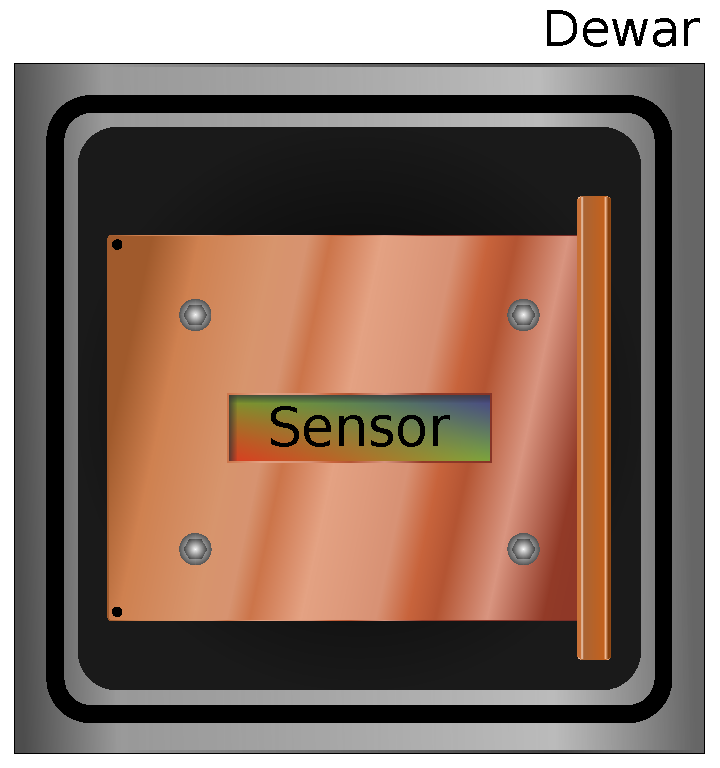
\includegraphics[scale=0.7]{Figs/Frontal_Dewar_Sensor.pdf}
    \caption{\footnotesize{Esquema frontal del Dewar y el posicionamiento del sensor. El sensor se encuentra montado detrás de una placa de cobre frontal con un abertura rectangular por donde la radiación incidente alcanza al sensor.}}
    \label{fig:FrontalDewarYSensor}
\end{figure}
Debido a las bajas temperaturas y para evitar la condensación de humedad dentro del recinto, se hizo vacío mediante la utilización de una bomba turbo-molecular, capaz de alcanzar una presión del orden de los $10^{-5}\,\si{mbar}$.\\
\indent También fue necesaria la utilización de un calentador para controlar la temperatura del sensor y del \textit{Dewar} por dos razones principales: Evitar que la temperatura de operación del sensor sea menor a $110\,\si{K}$, debido a que la eficiencia de la transferencia de carga entre píxeles del sensor se ve disminuida para temperaturas menores a esta; y para regular la velocidad de enfriamiento del sensor, dado que podría comprometerse el funcionamiento del mismo si esta superaba $1\,\si{K/s}$.\\
\subsection{Detector utilizado}
\noindent El detector utilizado fue un \textit{fully-depleted} CCD, del tipo \textit{bulk-iluminated}, es decir, que se expone a la radiación incidente una de sus lados y luego las cargas generadas se migran hacia el lado contrario. La zona muerta en la parte trasera del CCD estaba compuesta por tres capas: Una capa de $\sim 20\,\si{nm}$ de óxido de indio y estaño (ITO, por sus siglas en inglés: \textit{Indium Tin Oxide}), una capa de $\sim 38\,\si{nm}$ de dióxido de circonio (ZrO$_{2}$) y una última capa de $\sim 100\,\si{nm}$ de dióxido de silicio (SiO$_{2}$). El CCD estaba dividido en cuatro cuadrantes, denominados OHDU, con un amplificador en la esquina de cada cuadrante, permitiendo la lectura en simultaneo de todos ellos. Cada cuadrante consiste en $2063$ filas y $500$ píxeles por fila, y cada píxel tenía una dimensión de $15\,\si{\mu m} \times 15\,\si{\mu m}$.
%se cubrió el detector con una cámara de cobre fría. Esta cámara se encontraba en contacto térmico con la pieza de cobre fría en la cual se encuentra montado el detector y actúa de aislamiento de la radiación de cuerpo negro originada por las paredes de alrededor.\\
\subsection{Fuente de Americio radioactivo}
%Los rayos $X_{K}$ emitidos luego de la captura electrónica del $\prescript{55}{}{\mbox{Fe}}$ son ampliamente usados para calibración de CCDs. Sus energías, conocidas con excelente precisión, pueden verse en la tabla \ref{tab:EnergiasXk}. 
\noindent Para las mediciones estudiadas en este trabajo, se utilizó una fuente radioactiva de $\prescript{241}{}{\mbox{Am}}$ electrodepositada, que emitía partículas alfa con energía de $\sim 5.6\,\si{MeV}$, una actividad de $1\,\si{\mu C}$ y un diámetro de $5\,\si{mm}$. Para obtener los rayos $X$ de fluorescencia del flúor y del aluminio, se colocó dentro del recinto de cobre que alberga el sensor una cinta de Teflón, material que contiene flúor, y una placa de aluminio. La fuente radioactiva se colocó debajo del \textit{Dewar}, del lado exterior, al cual se le hizo un agujero por donde ingresaban las partículas alfa que impactarían los materiales para producir la fluorescencia.
\begin{figure}%[h]
    \centering
    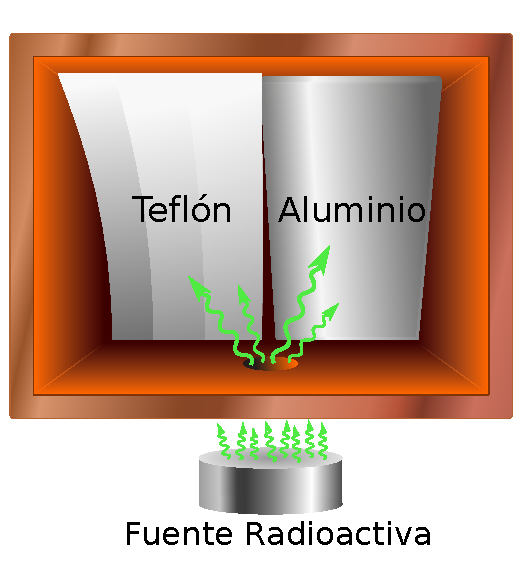
\includegraphics[scale=0.7]{Figs/CajaSensor.pdf}
    \caption{\footnotesize{Esquema frontal de la caja de cobre donde se posicionaron la cinta de teflón y la placa de aluminio. Se esquematiza el orificio por donde ingresan las partículas alfa, pero no la barrera allí colocada. El sensor se encuentra montado frente de esta, detrás de la placa de cobre del esquema de la figura \ref{fig:FrontalDewarYSensor}, de forma que los rayos de fluorescencia producidos por el aluminio y el teflón impacten sobre él.}}
    \label{fig:FrontalAlYF}
\end{figure}
Además, se colocó una pequeña barrera de cobre entre el orificio la fuente y el sensor para que las partículas alfa no llegasen directamente hacia este.
\begin{figure}%[h]
    \centering
    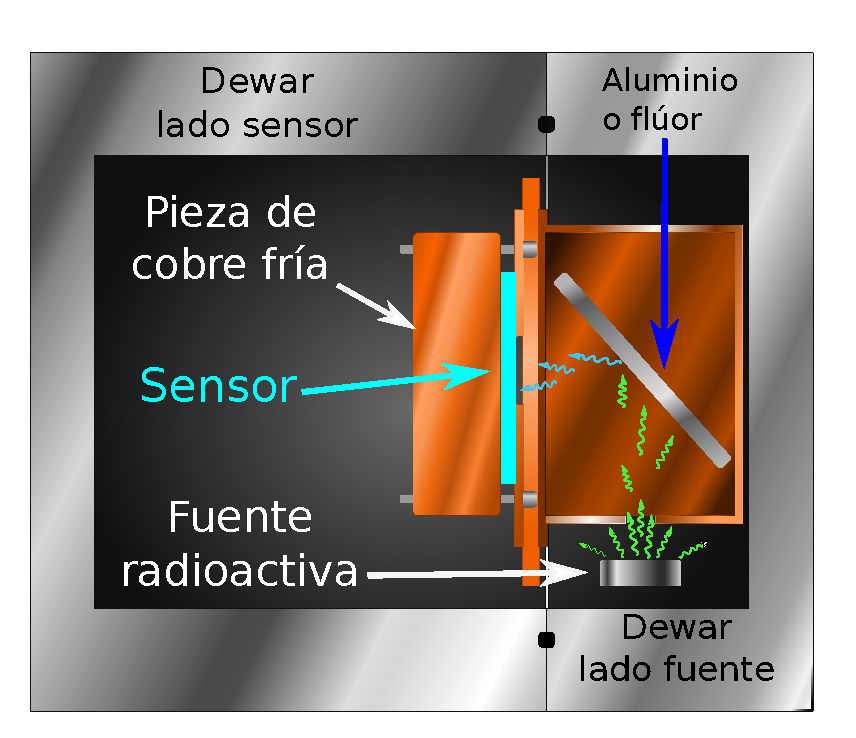
\includegraphics[scale=0.7]{Figs/LateralDewar.pdf}
    \caption{\footnotesize{Esquema lateral del \textit{Dewar}. Del lado izquierda se encuentra la placa de cobre con la abertura para el sensor (vista lateral del esquema \ref{fig:FrontalDewarYSensor}) el cual está en contacto con una pieza de cobre fría para mantenerlo en, por ejemplo, $123\,\si{K}$. Del lado derecho se encuentra la caja de cobre con la pieza de aluminio o de flúor, posicionada en ángulo y por encima del orificio por donde pasan las partículas alfa de la fuente radioactiva (vista lateral del esquema \ref{fig:FrontalAlYF}).}}
    \label{fig:LateralDewar}
\end{figure}
%\indent En una fracción importante de los decaimientos del $\prescript{55}{}{\mbox{Fe}}$, la energía es transferida a electrones en otros orbitales en vez transferirse como emisión de rayos $X$. Estos electrones \textit{auger} abandonan los átomos con unos pocos $\si{eV}$ menos que los rayos $X$ debido a la energía de ionización y crean un espectro continuo de energía cuando interactúan con el CCD. Para evitar este fondo, se cubrió la fuente de $\prescript{55}{}{\mbox{Fe}}$ con $20\,\si{\mu m}$ de \textit{Mylar}, que logran frenar los electrones con esta energía y además tienen una muy baja probabilidad de producir dispersión por efecto Compton de los rayos $X$. El ancho total de las capas de material que cubren al sensor es de $160\,\si{\mu m}$, sin embargo, se induce una probabilidad de interacción con los fotones de $5.9\,\si{keV}$ de $\sim 1.4 \%$.\\
%%%%%%%%%%%%%%%%%%%%%%%%%%%%%%%%%%%%%%%%%%%%%%%%%%%%%%%%%%%%%%%%%%
%%%%%%%%%%%%%%%%%%%%%%%%%%%%%%%%%%%%%%%%%%%%%%%%%%%%%%%%%%%%%%%%%%
\section{Mediciones}
%Para reducir el impacto de las corrientes oscuras se limitó la exposición y el tiempo de lectura al realizar la medición simultánea de los $4$ cuadrantes del CCD y restringiendo la adquisición a $50$ filas por cuadrante. 
\noindent Debido a que la tasa de eventos de fluorescencia de aluminio y flúor producidos fue relativamente baja, las colección de eventos se realizó exponiendo el detector durante $20$ minutos antes de realizar la medición de la carga en los píxeles. El sensor contiene $500$ píxeles por fila, donde $7$ píxeles son de \textit{pre-scan}, $443$ de región activa y $50$ de \textit{over-scan}. Se utilizaron solamente $50$ filas del sensor, con lo cual, el área activa de las imágenes fue de $22150$ píxeles. %La exposición a los rayos $X$ se realizó moviendo rápidamente las cargas en esos píxeles ($\sim 30\,\si{s}$ de exposición efectiva) de forma de conseguir una frecuencia de impacto de rayos $X$ de $\sim 4\,\si{Hz}$ en la región activa de cada imagen, resultando en $\sim 120$ eventos en promedio. 
Se realizaron $300$ mediciones por píxel, lo que corresponde a un tiempo de lectura de $\sim 10$ minutos por imagen.\\
\indent Luego de la lectura, las $300$ mediciones tomadas para cada píxel fueron promediadas y los píxeles vacíos del \textit{over-scan} fueron usados para calcular y extraer la linea de base de cada fila. Este proceso es necesario para la calibración, para poder establecer el valor en ADU's correspondiente al $0$ de carga para cada una de las filas del sensor. Las regiones de \textit{pre-scan} y \textit{over-scan} son regiones del sensor que no están colectando carga junto con la región activa, pero cuando se realiza la medición de los píxeles y las cargas son desplazadas secuencialmente, estos píxeles tiene una probabilidad muy baja (aunque no nula) de colectar algún evento al desplazarse hacia el nodo de sensado. Esa baja probabilidad de colectar carga durante el proceso de lectura es la razón por la cual esos píxeles son utilizadas para definir la linea de base de cada fila.\\
\indent Las imágenes resultantes contienen $443 \times 50$ píxeles por cada cuadrante y la carga es medida en unidades electrónico digitales (ADU's), que posteriormente fueron convertidas en electrones usando la calibración absoluta del sensor.\\
\indent Al final de cada ciclo de exposición/lectura, toda la carga colectada por el CCD era removida en un rápido proceso que toma aproximadamente un segundo.\\
\indent Los datos obtenidos durante el proceso de medición se almacenan como una imagen de formato \verb|.fits|. Cada píxel de esa imagen representa una medición del nodo de sensado. Debido a que gracias a la tecnología \textit{Skipper}-CCD es posible realizar la medición de carga de un píxel del sensor tantas veces como se deseé, si se tomó un número $N$ de muestreos por cada píxel del sensor, entonces la imagen \verb|.fits| tendrá $N$ píxeles por cada píxel real del sensor. Por esta razón, resulta necesario procesar la imagen para promediar los $N$ muestreos por píxel y así obtener una lectura real de carga y con muy bajo ruido de lectura, a la vez de disminuir drásticamente el tamaño y peso de la imagen. Esta última imagen es la que contiene los datos relevantes para este trabajo.